\section{Background Literature}
Summary. This section deals with literature found in books.

\subsection{Probability Theory}
The calculus of Probability Theory was developed by Fermat and Pascal in order to better understand the problems introduced by uncertainty in gambling. From this dubious genesis a rich and incredibly powerful field has developed. We start our brief introduction of probability theory by restating Kolmogorov's three probability axioms - these axioms underpin the entire theory of probability.

Let the set $\Omega$ be the universe of possible events, also called the event space; that is, if we are uncertain about which of a number of possibilities are true then we let $\Omega$ represent all of them collectively. Let $P$ be some real valued function which satisfies the three axioms stated below.
\begin{ax}
$P(\Omega) = 1$. The probability of any event in $\Omega$ occurring is 1.
\end{ax}
\begin{ax}
$\forall \alpha \in \Omega,~P(\alpha) \geq 0$. The probability of any one (or set of) event(s) in $\Omega$ occurring is non-negative. 
\end{ax}
\begin{ax}
$\forall \alpha, \beta \in \Omega,\text{ if } \alpha \cap \beta = \emptyset \text{ then } P(\alpha \cup \beta) = P(\alpha) + P(\beta)$. The probability of two mutually disjoint sets of events in $\Omega$ occurring is equal to the sum of their probabilities.
\end{ax}
A function $P$ which satisfies these three axioms is known as a probability function. Based on these three axioms we are able to extend the theory to Theorem \ref{thrm_prob_union_intersect}.
\begin{thrm}
$\forall \alpha, \beta \in \Omega, P(\alpha \cup \beta) = P(\alpha) + P(\beta) + P(\alpha \cap \beta)$. The probability of two events occurring in $\Omega$ is equal to the sum of their probabilities less the probability of both occurring simultaneously.
\label{thrm_prob_union_intersect}
\end{thrm}

\subsubsection{Discrete Random Variables}

We now make precise what we mean by random variables: a random variable is a non-deterministic variable which is characterised by some uncertainty in its measurement. Semantically we indicate a specific value taken on by the random variable $X$ as $X=x$ or just denote it $x$. Thus, the function $P(X=x)=P(x) \in \mathbb{R}$ indicates the probability of event $x$ occurring with respect to the random variable $X$. We denote $P(X)$ as the probability function of the random variable $X$. Thus, for the discrete random variable $X$ we have that $P(X)=(P(x_1),P(x_2),...,P(x_n))^T$ where $x_i \in X$ for $i=1,2,..., n$ and $\sum_i P(x_i) =1$. We defer the study of the continuous case until later.

Before we proceed let us briefly discuss how we can interpret the function $P$ for any random variable $X$. If $P(X=x)=1$ we are certain of event $x$ occurring, i.e. $X$ will only take on the value $x$. If $P(x)=0$ we are certain that event $x$ will not occur, i.e. $X$ will never take on the value $x$. Thus our certainty of event $x$ occurring is reflected by the magnitude of $P(x)$. Attempting to make the statement ``our certainty of event $x$ occurring" more precise leads us to two different physical interpretations of $P(x)$. The first is the frequentist interpretation: to the frequentist a probability is a long term average of the observations of event $x$ occurring in the event space. While this interpretation is satisfying if one deals with something which is easily measured e.g. the probability of a fair die rolling a 6, it fails to explain statements like: ``the probability of it raining tomorrow is 50\%". The reason the last statement is problematic is because the time span is ill defined. If we rather understand probabilities to mean subjective degrees of belief in event $x$ occurring this is no longer a problem. To ensure that these subjective beliefs are rational can be problematic. One way to ensure this is by requiring that if the probabilities were used in a betting game it is impossible to exploit them to one's advantage (or disadvantage). If this is possible then there is no difference between the interpretations described above \cite{koller}. 

We will deal extensively with joint and marginal probability distributions. Consider the random variables $X$ and $Y$. The marginal probability distribution of $X$ is the function $P(X)$ and describes the probabilities of events involving only the variable $X$. The joint probability distribution of $X$ and $Y$ is the function $P(X,Y) = P(X \cap Y)$ and describes the intersection (and) of the probability space of $X$ and $Y$. We introduce, without proof, Theorem \ref{thrm_marg}.
\begin{thrm}
\textbf{Marginalisation} By marginalising out $X$ we mean we sum out $X$ from the joint distribution $P(Y) = \sum_x P(x, Y)$. This extends to higher dimensions. 
\label{thrm_marg}
\end{thrm}
We can reduce any joint distribution to a marginal one by summing (or integrating in the case of continuous random variables) out the appropriate variable. 

It is now necessary to define what we mean by conditional probability. Definition \ref{defn_cond_prob} makes precise how the knowledge that event $y$ has occurred alters our view of event $x$ occurring.  
\begin{defn}
\textbf{Conditional Probability} $P(X|Y) = \frac{P(X \cap Y)}{P(Y)}$ 
\label{defn_cond_prob}
\end{defn}
Note that if for some $y \in Y$ we have $P(Y=y) = 0$ then Definition \ref{defn_cond_prob} is undefined. Additionally, the function $P(\cdot|Y)$ is a probability function. We next define what we mean by a positive probability distribution in Definition \ref{defn_pos_distr}.
\begin{defn}
A probability distribution is positive if $P(x) > 0~\forall~x \in X$.
\label{defn_pos_distr}
\end{defn}
Clearly undefined conditional probabilities are not a problem in the setting of positive probability distributions. We also define the notion of independence, also sometimes called marginal independence, in Definition \ref{defn_indep}. 

As before, let $X$, $Y$ and $Z$ be random variables. Intuitively $X$ and $Y$ are independent if the outcome of $X$ does not influence the outcome of $Y$. It can be shown that independence is a symmetric property \cite{koller}.
\begin{defn}
\textbf{Independence} $X \indep Y \equiv P(X|Y) = P(X)$ 
\label{defn_indep}
\end{defn}
Generalising the concept of independence we define conditional independence by Definition \ref{defn_cond_indep}. Again this definition is symmetric \cite{koller}.
\begin{defn}
\textbf{Conditional Independence} $X \indep Y | Z \equiv P(X|Y,Z) = P(X|Z)$
\label{defn_cond_indep}
\end{defn}
Intuitively, if $X$ is conditionally independent of $Y$ given $Z$ then by observing $Z$ one gains nothing by observing $Y$. Clearly if $Z=\emptyset$ we have (marginal) independence. We also introduce Theorem \ref{thrm_chain_rule} which naturally leads us to the formulation of Bayes' Theorem (using Definition \ref{defn_cond_prob}) as shown in Theorem \ref{thrm_bayes}. 
\begin{thrm}
\label{thrm_chain_rule}  
\textbf{Chain Rule} Given the random variables $X_1$ and $X_2$ we have $P(X_1,X_2) = P(X_1)P(X_2|X_1)$. The generalisation to an arbitrary number of random variables is straightforward.
\end{thrm}
\begin{thrm}
\textbf{Bayes' Theorem} $P(X|Y) = \frac{P(Y|X)P(X)}{P(Y)}$
\label{thrm_bayes}
\end{thrm}
Under the Bayesian interpretation of Theorem \ref{thrm_bayes} we see that the posterior probability of some hypothesis $X$ given some evidence $Y$ being true is just the likelihood $P(Y|X)$ of the hypothesis supporting the evidence multiplied by the prior probability of the hypothesis $P(X)$ normalised by the prior of the evidence $P(Y)$. It is also convenient to notice that $P(Y)$ is a normalising constant and thus  $P(X|Y) \propto P(Y|X)P(X)$.

To fully describe a system of random variables it is only necessary to know the joint distribution $P(X_1,X_2,...,X_n)$. Given the joint probability distribution inference (reasoning about the variables under uncertainty) may be performed. Common probabilistic queries involve computing posterior beliefs $P(X|Y=y)$ i.e. the probability function of $X$ given we have some information about $Y$. Other queries involve find the most probable explanation (called a MAP query) of some evidence i.e. finding $X$ which maximises $P(X, Y=y)$. More on this later. 

\textbf{Bayes' Theorem: Example}\\
This section will attempt to develop some intuition behind Theorem \ref{thrm_bayes}. We quote an excerpt from an article in the Economist \cite{eco1} and illustrate the use of Bayes' Rule in a canonical medical example \cite{korb}.

\textit{``The essence of the Bayesian approach is to provide a mathematical rule explaining how you should change your existing beliefs in the light of new evidence. In other words, it allows scientists to combine new data with their existing knowledge or expertise. The canonical example is to imagine that a precocious newborn observes his first sunset, and wonders whether the sun will rise again or not. He assigns equal prior probabilities to both possible outcomes, and represents this by placing one white and one black marble into a bag. The following day, when the sun rises, the child places another white marble in the bag. The probability that a marble plucked randomly from the bag will be white (ie, the child's degree of belief in future sunrises) has thus gone from a half to two-thirds. After sunrise the next day, the child adds another white marble, and the probability (and thus the degree of belief) goes from two-thirds to three-quarters. And so on. Gradually, the initial belief that the sun is just as likely as not to rise each morning is modified to become a near-certainty that the sun will always rise."}

Suppose you get tested for a certain disease. You know the disease affects 1 in 100 people. You also know that the false positive rate for the test is 20\% and the false negative rate for the test is is 10\%. Your test comes back positive. What are the chances of you having the disease given this information?

The information may be summarised as shown below. Let $D$ be a binary random variable indicating the presence of the disease and $\neg D$ indicates the absence. Let $T$ be a binary random variable indicating a positive test and $\neg T$ indicates a negative test. 
\begin{enumerate}
\item
The prior of the disease is $P(D) = 0.01$.
\item
False positive rate $P(T|\neg D) = 0.2 \implies P(\neg T|\neg D) = 0.8$.
\item
False negative rate $P(\neg T|D) = 0.1 \implies P(T|D) = 0.9$.
\end{enumerate}
A naive approach would conclude that since $P(T|D) = 0.9$ you are 90\% likely to have the disease. However, using Bayesian inference/reasoning we have: 
\begin{equation*}
\begin{aligned}
P(D|T) &= \frac{P(T|D)P(D)}{P(T)} \\
&=  \frac{P(T|D)P(D)}{\sum_D P(D,T)} \\
&= \frac{P(T|D)P(D)}{\sum_D P(D)P(T|D)} \\
& = \frac{0.9 \times 0.01}{0.01 \times 0.99 + 0.99 \times 0.2} \\
&\approx 0.04
\end{aligned}
\end{equation*}
Clearly there is a big difference between the naive approach and the Bayesian (correct) approach. The power of Bayesian inference lies in the ability to reverse causal reasoning. That is, we know that the disease causes the test to be positive, $P(T|D)$, but we would like to reverse this reasoning to infer $P(D|T)$. This is immensely powerful as we shall soon discover.   

\subsubsection{Continuous Random Variables}

So far in our discussion we have implicitly only used discrete random variables; that is, our probability space consisted out of a finite number of events or states. However, it is also necessary to make precise what we mean by a continuous random variable. A continuous random variable is characterised by a density function $p$ which assigns a weight to each possible value of the variable. Intuitively this weight is \underline{related} to the ``probability" of that value occurring\footnote{Please note that strictly speaking $P(x)=0$ for a specific point $x$ in the domain of $p$. Technically it is correct to say that the probability of $P(x \in [a,b]) = \int_a^b p(y)dy$; thus, if we want the probability of $x$ occurring we could just make $[a,b]$ small.}. Although the density function is itself not a probability function, if it satisfies $p(x) \geq 0~\forall x \in X$ and $\int p(x)dx = 1$, where we have implicitly integrated over the domain of $p$, then it can be used to generate one. The cumulative probability function $P(X \leq a)=\int^a_{-\infty} p(x)dx$ is one such example\footnote{We have assumed that the domain of $X$ is the entire real line.}. 

Arguably the most well known continuous probability density distribution is the Gaussian or Normal distribution. The Gaussian distribution arises naturally from a variety of different contexts and settings. For example, the central limit theorem, together with some mild assumptions, tells us that the sum of a set of $N$ random  variables is itself a random variable and in the limit can be described by a Gaussian distribution \cite{bishop}. The Gaussian is regularly used because it has some very appealing analytical properties (and often also because it is physically meaningful) which we will investigate in some depth. 

Since the probability of a specific value is not meaningful in the setting of continuous probability functions we abuse our notation and denote the random variable $X$ by $x$. We also do not indicate vector quantities in boldface. We will concern ourselves mostly with vector quantities and it will be obvious when we deal with non-vector valued variables. 
\begin{defn}
\textbf{Gaussian Distribution} The univariate Gaussian or Normal distribution of a random variable $x$ is shown in (\ref{eq_norm_uni}). We call $\mu$ the mean and $\sigma^2$ the variance of the distribution.
\begin{equation}
\mathcal{N}(x|\mu, \sigma^2) = \frac{1}{\sqrt{2\pi\sigma^2}}\exp\left(-\frac{1}{2\sigma^2}(x-\mu)^2\right)
\label{eq_norm_uni}
\end{equation}
The multivariate Gaussian distribution is shown in (\ref{eq_norm_multi}) where $\mu$ is a $D$ dimensional mean vector and $\Sigma$ is a $D \times D$ dimensional covariance matrix. Note that we often use the inverse of the covariance matrix, called the precision matrix and define it $\Lambda \equiv \Sigma^{-1}$.
\begin{equation}
\mathcal{N}(x|\mu, \Sigma) = \frac{1}{\sqrt{2\pi^{\frac{D}{2}}}}\frac{1}{|\Sigma|^{\frac{1}{2}}}\exp\left(-\frac{1}{2}(x-\mu)^T\Sigma^{-1}(x-\mu)\right)
\label{eq_norm_multi}
\end{equation}
\label{defn_gauss}
\end{defn}
It is also appropriate to define some functions which apply equally well to the discrete case as to the continuous case (just replace the integration with summation in the setting of discrete random variables). We define the expectation (or mean or average) in Definition \ref{def_expectation}, the variance in Definition \ref{def_variance} and the covariance in Definition \ref{def_covariance}. 
\begin{defn}
\textbf{Expectation} The average value of some integrable function $f$ under the probability distribution $p$ is denoted $\mathbb{E}[f] = \int p(x)f(x)dx$.
\label{def_expectation}
\end{defn}
We have that $\mathbb{E}[x]=\mu$ if $x$ is a Gaussian random variable.
\begin{defn}
\textbf{Variance} The variance of $f$ is defined by $\text{var}[f] = \mathbb{E}[(f - \mathbb{E}[f])^2]$ and provides a measure of how much variability there is in $f$ around its mean value $\mathbb{E}[f]$.
\label{def_variance}
\end{defn}
By expanding out the square we have the familiar formulate $\text{var}[f] = \mathbb{E}[f^2] - \mathbb{E}[f]^2$. Also note that for a  univariate Gaussian random variable $x$ we have $\text{var}[x] =\sigma^2$.
\begin{defn}
\textbf{Covariance} For two random variables $x,y$ (which may be vectors) we define the covariance matrix $\text{cov}[x,y] = \mathbb{E}[xy^T] - \mathbb{E}[x]\mathbb{E}[y]$.
\label{def_covariance}
\end{defn}
Note that $\text{cov}[x,x]=\text{cov}[x]=\text{var}[x]$. Covariance is a measure of how much two random variables vary together. If $x$ is a $D$ dimensional Gaussian random variable then $\text{cov}[x] = \Sigma$ as defined in Definition \ref{defn_gauss}.

The identities in Theorem \ref{thrm_gaussian_identities} will be useful in later sections. We refer the reader to \cite{davidian} for justification.
\begin{thrm}
\textbf{Gaussian Expected Value Identities}
Suppose there exist constants $c \in \mathbb{R}^n$ and $C \in \mathbb{R}^{n \times n}$ and $X$ is a normal random variable with statistics $(\mu, \Sigma)$. Then the following identities hold:
\begin{enumerate}
\item
$\mathbb{E}[c^TX] = c^T\mu$
\item
$\mathbb{E}[CX+c] = C\mu + c$
\item
$\mathbb{E}[X^TCX] = \text{tr}(C\Sigma) + \mu^TC\mu$
\end{enumerate}
\label{thrm_gaussian_identities}
\end{thrm}  

Now we are in a position to perform some manipulations assuming we are using Gaussian random variables. We state without proof Theorem \ref{thrm_joint_gaussians}.
\begin{thrm}
\textbf{Partitioned Joint Gaussians}
Given a Gaussian distribution $\mathcal{N}(x|\mu,\Sigma)$ with $\Lambda \equiv \Sigma^{-1}$ and $x=\begin{pmatrix}
x_a \\ x_b
\end{pmatrix}$, $\mu=\begin{pmatrix}
\mu_a \\ \mu_b
\end{pmatrix}$, $\Sigma=\begin{pmatrix}
\Sigma_{aa} & \Sigma_{ab} \\ \Sigma_{ba} & \Sigma_{bb}
\end{pmatrix}$ and $\lambda = \begin{pmatrix}
\Lambda_{aa} & \Lambda_{ab} \\ \Lambda_{ba} & \Lambda_{bb}
\end{pmatrix}$ then we have the conditional distribution in (\ref{eq_part_joint_gauss1}) and the marginal distribution in (\ref{eq_part_joint_gauss2}).
\begin{equation}
\begin{aligned}
&p(x_a|x_b) = \mathcal{N}(x_a|\mu_{a|b}, \Lambda_{aa}^{-1}) \\
&\text{with } \mu_{a|b} = \mu_a - \Lambda_{aa}^{-1}\Lambda_{ab}(x_b-\mu_b)
\end{aligned}
\label{eq_part_joint_gauss1}
\end{equation}
\begin{equation}
p(x_a) = \mathcal{N}(x_a|\mu_a,\Sigma_{aa})
\label{eq_part_joint_gauss2}
\end{equation}
\label{thrm_joint_gaussians}
Note that for the conditional distribution it is easier to work with the precision matrix. 
\end{thrm}
Next we state and then prove Theorem \ref{thrm_bayes_gaussians} which we will use extensively. The proof for Theorem \ref{thrm_joint_gaussians} uses the same techniques and can be found in \cite{bishop}.
\begin{thrm}
\textbf{Bayes' Theorem for Linear Gaussian Models}
Suppose we have a marginal Gaussian distribution for $x$ and a conditional Gaussian distribution for $y$ in the form shown in (\ref{eq_bayes_gauss_suppose}).
\begin{equation}
\begin{aligned}
p(x) &= \mathcal{N}(x|\mu,\Lambda^{-1}) \\
p(y|x) &= \mathcal{N}(y|Ax + b, L^{-1}) 
\end{aligned}
\label{eq_bayes_gauss_suppose}
\end{equation} 
Then the marginal distribution for $y$ is given by (\ref{eq_bayes_gauss1}) and the conditional distribution for $x$ given $y$ is (\ref{eq_bayes_gauss2}).
\begin{equation}
p(y) = \mathcal{N}(y|A\mu + b, L^{-1}+A\Lambda^{-1}A^T)
\label{eq_bayes_gauss1}
\end{equation}
\begin{equation}
\begin{aligned}
&p(x|y) = \mathcal{N}(x|\Sigma(A^TL(y-b)+\Lambda\mu), \Sigma) \\
&\text{with } \Sigma = (\Lambda + A^TLA)^{-1}
\end{aligned}
\label{eq_bayes_gauss2}
\end{equation}
\label{thrm_bayes_gaussians}
Note that $b$ is a known vector. Given a deterministic function $u$ we can also write $b = Bu + e$ where $B$ is some conforming matrix and $e$ is some constant vector. 
\end{thrm}
\begin{proof}
We begin our proof by noticing that for a general Gaussian $\mathcal{N}(\gamma|\alpha, \beta)$ we can write the exponent as in (\ref{eq_bg1}), note $const$ is some real number which does not depend on $\gamma$.
\begin{equation}
-\frac{1}{2}\left(\gamma-\alpha \right)^T\beta^{-1}\left(\gamma-\alpha \right) = -\frac{1}{2}\gamma^T\beta^{-1}\gamma +\gamma^T\beta^{-1}\alpha + const
\label{eq_bg1} 
\end{equation}
Also note that Gaussian distributions are closed under multiplication, i.e. if one multiplies two Gaussian distributions the product is still a Gaussian distribution (of a higher dimension). To find the joint distribution we let $z = \begin{pmatrix}
x \\ y
\end{pmatrix}$ and consider the log of the joint in (\ref{eq_log_gauss_joint}).
\begin{equation}
\begin{aligned}
\log(z) &= \log(p(x)) + \log(p(y|x))\\
&=  -\frac{1}{2}(x-\mu)^T\Lambda(x-\mu) -\frac{1}{2}(y-Ax-b)^T L(y-Ax-b) + const
\end{aligned}
\label{eq_log_gauss_joint}
\end{equation}
Here $const$ denotes constant terms which are independent of $x$ and $y$. Now we make use of (\ref{eq_bg1}) to find the mean and covariance of $z$. Continuing, we consider only the second order terms when (\ref{eq_log_gauss_joint}) is expanded, as shown in (\ref{eq_gauss_joint_precision}).
\begin{equation}
\begin{aligned}
&-\frac{1}{2}x^T(\Lambda+A^TLA)x-\frac{1}{2}y^TLy + \frac{1}{2}y^TLAx+\frac{1}{2}x^TA^TLy \\
&= -\frac{1}{2}\begin{pmatrix}
x \\ y
\end{pmatrix}^T \begin{pmatrix}
\Lambda+A^TLA & -A^TL \\ -LA & L
\end{pmatrix}\begin{pmatrix}
x \\ y
\end{pmatrix} \\
&= -\frac{1}{2}z^TRz
\end{aligned}
\label{eq_gauss_joint_precision}
\end{equation}
From this we immediately have the precision of $z$: the matrix $R$; we also use a matrix inversion formula found in \cite{bishop} to find the covariance. This is shown in (\ref{eq_gauss_covar}).
\begin{equation}
\text{cov}[z] = R^{-1} = \begin{pmatrix}
\Lambda^{-1} & \Lambda^{-1}A^T \\ A\Lambda^{-1} & L^{-1}+A\Lambda^{-1}A^T
\end{pmatrix}
\label{eq_gauss_covar}
\end{equation}
We now proceed in exactly the same way to find mean of $z$. By expanding \ref{eq_log_gauss_joint} and only considering the first order terms in $x$ and $y$ we have (\ref{eq_gauss_mean1}).
\begin{equation}
x^T\Lambda\mu-x^TA^TLb+y^TLb = \begin{pmatrix}
x \\ y
\end{pmatrix}\begin{pmatrix}
\Lambda\mu - A^TLb \\Lb
\end{pmatrix}
\label{eq_gauss_mean1}
\end{equation}
Again, by making use of (\ref{eq_bg1}) and the fact that the covariance of $z$ is $R^{-1}$ it is possible to show that $\mathbb{E}[z]=\begin{pmatrix}
\mu \\ A\mu +b
\end{pmatrix}$ as shown in \cite{bishop}. By using Theorem \ref{thrm_joint_gaussians} we immediately have the marginal and conditional distributions as required.
\end{proof}

\subsection{Graph Theory}
A graph, $G$, is a data structure consisting of a set of nodes $\chi$ and edges $\xi$. A pair of nodes $X_i, X_j \in \chi$ can be connected by an edge. We will only consider directed graphs in this dissertation. This implies that every edge in $\xi$ has a direction associated between the two nodes it connects i.e. $X_i \rightarrow X_j$ if there is an edge from $X_i$ to $X_j$.

We now define some basic concepts which we will rely upon to further describe the types of graphs we will consider.
\begin{defn}
\textbf{Directed Path} We say that the nodes $X_1, X_2, X_3,..., X_n \in \chi$ form a directed path if $X_i \rightarrow X_{i+1}$ for $1 \leq i \leq n-1$. 
\end{defn}
\begin{defn}
\textbf{Directed Cycle} A directed cycle is a non-singleton directed path which starts and ends at the same node.
\end{defn}
\begin{defn}
\textbf{Directed Acyclic Graph (DAG)} A graph $G$ is a DAG if it is directed and has no directed cycles.
\end{defn}
In this dissertation we will only concern ourselves with DAGs. Figure \ref{fig_dag} is an example of a DAG.
\begin{figure}[H] 
\centering
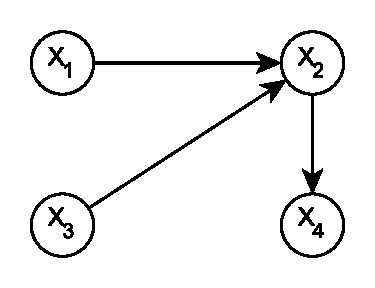
\includegraphics[scale=1.0]{dag.pdf}
\caption{Example of a Directed Acyclic Graph}
\label{fig_dag}
\end{figure}
Next we define some nomenclature to further describe the nodes of a graph $G$.
\begin{defn}
\textbf{Parents} We say that the set of nodes $\kappa \subset \chi$ are the parents of node $X_i$ if, for each node in $\kappa$, there exists an edge going to $X_i$.
\end{defn}
\begin{defn}
\textbf{Children} We say that the set of nodes $\tau \subset \chi$ are the children of node $X_i$ if, for each node in $\tau$, there exists an edge going from $X_i$ to that node.
\end{defn}
\begin{defn}
\textbf{Descendants} We say that the set of nodes $\gamma \subset \chi$ are the descendants of node $X_i$ if, for each node in $\gamma$, there exists a directed path from $X_i$ to that node.
\end{defn}
We also briefly define a structured approach to encoding a graph.
\begin{defn}
\textbf{Adjacency Matrix} For a graph $G$ with $n$ nodes, the adjacency matrix $A$ is an $n \times n$ matrix where $A_{ij} = 1$ if there is an edge from node $i$ to node $j$ and $A_{ij} = 0$ otherwise. 
\end{defn}
The adjacency matrix A for Figure \ref{fig_dag} is shown below:
\begin{equation*}
A = \begin{pmatrix}
0 & 1 & 0 & 0 \\
0 & 0 & 0 & 1 \\
0 & 1 & 0 & 0 \\
0 & 0 & 0 & 0
\end{pmatrix}
\end{equation*}

A detailed analysis of Graph Theory may be found in \cite{deo}.

\subsection{Probabilistic Graphical Models}
Probabilistic graphical models are the union between Probability Theory and Graph Theory. Consider why, in general, it is infeasible to determine an arbitrary joint probability distribution. Suppose you have a set of $n$ binary random variables and wish to determine their joint. This equates to finding $P(X_1,X_2,...,X_n)$. To fully specify this model we would need to find and store $2^n-1$ probabilities. For even moderately big $n$ this is impractical, and this was for the simple case of a binary valued random variable. Clearly we require a more efficient way to represent the joint probability distribution.

\subsubsection{Bayesian Networks}
A Bayesian Network is a representation of the joint probability distribution of a set of random variables parametrised by:
\begin{enumerate}
\item
A graph depicting local independence relationships.
\item
Conditional probability distributions.
\end{enumerate}  
The fundamental assumption behind Bayesian Networks, and more generally probabilistic graphical models, is that there is a useful underlying structure to the problem being modelled which can be captured by the Bayesian network. This underlying structure is available via conditional independence relationships between the variables.

Suppose $P$ is the joint distribution of some set of random variables we require to do inference on.
\begin{defn}
\textbf{I-Map} The I-Map of $P$, denoted by $\mathcal{I}(P)$, is the set of independence assertions of the form $X \indep Y | Z$ which hold over $P$.
\end{defn} 
Let $G$ be a Bayesian Network graph over the random variables $X_1, X_2,...,X_n$ where each random variable is a node. We say that the distribution $P$ factorises over the same space if $P$ can be expressed as the product defined by the chain rule for Bayesian Networks.
\begin{defn}
\textbf{Chain Rule for Bayesian Networks} The chain rule for Bayesian Networks specifies that the joint factorises according to $P(X_1,...,X_n) = \Pi_{i=1}^n P(X_i | \text{Parents}(X_i))$.
\end{defn}
Each of the individual factors of $P$, as factorised by the chain rule for Bayesian Networks, represents the conditional probability distributions required to parametrise the Bayesian Network. It can be shown that a Bayesian Network graph $G$ over which $P$ factorises is not unique. However, if the graph explicitly models the causality inherent in the system being modelled the representation is often much sparser \cite{koller}. A Bayesian network is then defined as the tuple $(G, P)$ such that the joint $P$ factorises over the graph $G$. We state without proof Theorem \ref{thrm_bayesnetsiff}. 
\begin{thrm}
Let $G$ be a Bayesian Network graph over a set of random variables $\chi$ and let $P$ be a joint distribution over the same space. If $P$ factorises according to $G$ then $G$ is an I-Map for P. Conversely, if $G$ is an I-Map for $P$ then $P$ factorises according to $G$.
\label{thrm_bayesnetsiff}
\end{thrm}
Thus, the conditional independences imply factorisation of $P$. Conversely, factorisation according to $G$ implies the associated conditional independences.

To illustrate computational benefit of using Bayesian networks, consider again our simple system of $n$ binary random variables $X_1,X_2,...,X_n$. Suppose the Bayesian Network in Figure \ref{fig_bnet} models the system.
\begin{figure}[H] 
\centering
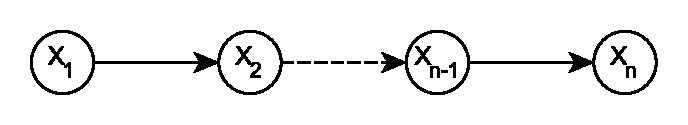
\includegraphics[scale=1.0]{bayes_net.pdf}
\caption{Example simple Bayesian Network}
\label{fig_bnet}
\end{figure}
Without knowing any structure $2^{n}-1$ parameters were needed to specify the joint. However, using the chain rule for Bayesian Networks we can factorise the joint $P(X_1,...,X_n) = P(X_1)P(X_2|X_1)...P(X_n|X_{n-1})$. This implies that we only require $2n-1$ parameters. From a modelling perspective this is a significant gain.

The primary reason we would want to have a model of the joint distribution of a set of random variables is to reason with. To achieve this we invariably manipulate the joint distribution by either some form of marginalisation or optimisation. To make inference computationally tractable it is desirable to leverage the independence assertions implied by the network graph. To this end we expand on the independence assertions implied by the graph. Recall Theorem \ref{thrm_bayesnetsiff}: since we have that the joint factorises over the graph we also have that any independence assertions implied by the graph's connectivity also apply to the joint.

We introduce the concept of d-separation as a method of determining whether a set of nodes $X$ are independent of another set $Y$ given the set $E$. Firstly we generalise the concept of a directed path to an undirected path between sets of variables.
\begin{defn}
\textbf{Undirected Path} An undirected path between two sets of nodes $X$ and $Y$ is any sequence of nodes between a member of $X$ and a member of $Y$ such that every adjacent pair of nodes is connected by an edge regardless of direction and no node appears twice.
\end{defn}
\begin{defn}
\textbf{Blocked Path} A path is blocked, given a set of nodes $\mathbf{E}$, if there is a node $Z$ on the path for which at least one of the three conditions holds:
\begin{enumerate}
\item
$Z$ is in $E$ and $Z$ has one edge leading into it from the path and one edge leading out of it on the path.
\item
$Z$ is in $E$ and $Z$ has both edges leading out of it from the path.
\item
Neither $Z$ nor any descendant of $Z$ is in $E$ and both path edges lead into $Z$.
\end{enumerate}
\end{defn}
\begin{defn}
\textbf{d-separation} A set of nodes $E$ d-separates two other sets of nodes $X$ and $Y$ if every path from a node in $X$ to a node in $Y$ is blocked given $E$.
\end{defn}
To shed some more light on d-separation consider Figure \ref{fig_dsep}. The first diagram depicts the first blocked condition, i.e. a causal chain. Node $E$ blocks relevance of $X$ to $Y$. The second diagram illustrates the second blocked condition, i.e. a common cause. Node $E$ blocks $X$ from being relevant to $Y$. Finally, the third diagram illustrates the third blocked condition or, more aptly, illustrates how lack of knowledge of the nodes in the path from $X$ to $Y$ implies that they are conditionally independent \cite{korb}.
\begin{figure}[H] 
\centering
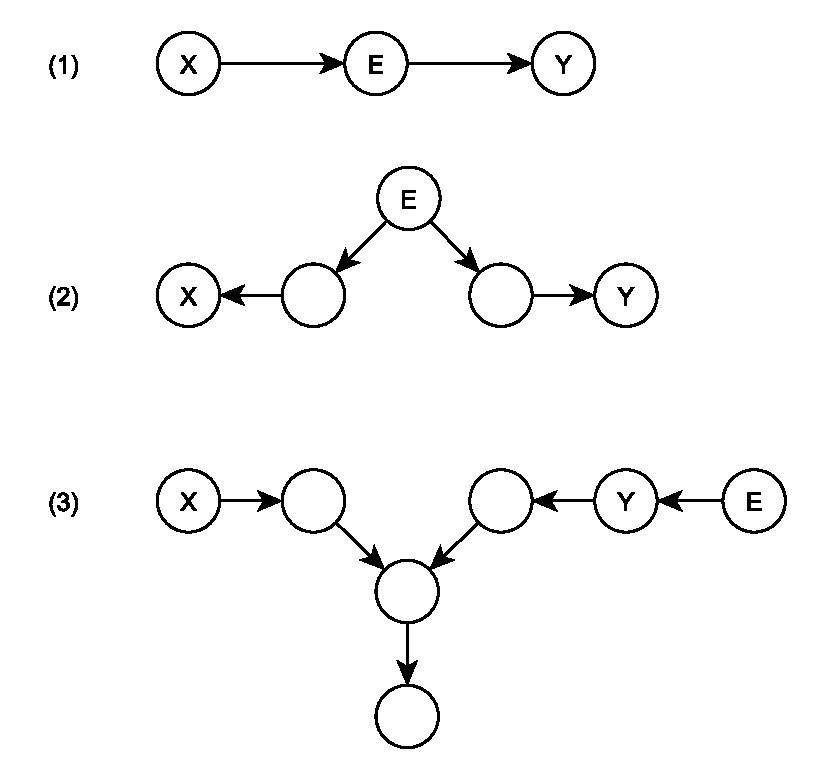
\includegraphics[scale=0.5]{dsep.pdf}
\caption{Examples of d-separation}
\label{fig_dsep}
\end{figure}
Using d-separation we can efficiently reason about the conditional independences implied by the graph and the observed variables ($E$). This becomes incredibly useful when one attempts to apply inference techniques because it can simplify the joint calculations significantly. More on this later.

Bayesian Networks are commonly used to model situations which are not time dependent. We will primarily restrict ourselves to time series modelling in this dissertation. As such we will not delve deeper into static Bayesian Network theory.

\subsubsection{Dynamic Bayesian Networks}
Dynamical Bayesian Networks generalise the conventional static Bayesian Networks of the previous section. Dynamic, or Temporal, Bayesian Networks model systems which evolve with time. Since sequential, or temporal, data is abundant in most engineering applications we will primarily concern ourselves with such models. Notationally we denote a time dependent vector by $x_{1:t}=x_1,x_2,...,x_t$, for example the joint $P(x_{1:3})=P(x_1,x_2,x_3)$.

There are two important classes of analysis one may perform on sequential data using graphical models. On-line analysis, including prediction and filtering and off-line analysis, including smoothing and the most probable explanation (sometimes called Viterbi decoding). In both cases we are generally interested in learning something about a set of hidden state variables by performing inference on some set of observed variables. 

A state space model assumes that there is some underlying hidden state ($X_t$) of the world which generates observations ($Y_t$). These hidden states may evolve with time and may be functions of some inputs ($U_t$). The hidden states and observations are most generally assumed to be random variables. Any state space model is fully parametrised by the following information:
\begin{enumerate}
\item
A prior probability distribution over the states: $P(X_1)$
\item
A state transition function: $P(X_t|X_{1:t-1}, U_{1:t-1})$
\item
An observation function: $P(Y_t|X_{1:t}, U_{1:t-1})$
\end{enumerate} 
For the purposes of this dissertation we will assume that the state space model is known. If this model is not known many machine learning techniques may be used find these models \cite{murphy1}. To simplify notation we will sometimes omit the dependence of the probability functions on the inputs $U_{1:t}$.

We will assume that all the systems we model satisfy the first order Markov assumption.
\begin{defn}
\textbf{N\textsuperscript{th}-order Markov assumption} A system satisfies the N\textsuperscript{th} Markov assumption if $P(X_t|X_{1:t})=P(X_t|X_{t-n:t-1})$. For example, a first order Markov system satisfies  $P(X_t|X_{1:t})=P(X_t|X_{t-1})$. Similarly with the observation function.
\end{defn}
This is not as restrictive as it may seem at first. It is always possible to transform an N\textsuperscript{th}-order Markov system into a first order Markov system by modifying the state space \cite{murphy1}. We also assume that the state and observation functions remain the same for all time i.e. they are time invariant or homogeneous or stationary.

Intuitively, a state space model is a model of how $X_t$ generates or causes $Y_t$ and $X_{t+1}$. The goal of inference is to invert this mapping. The four types of inference we will consider in this dissertation are:
\begin{enumerate}
\item
Filtering: we attempt to infer $P(X_t|y_{1:t})$, i.e. we attempt to estimate the current state given all past observations.
\item
Smoothing: we attempt to infer $P(X_{t-m}|y_{1:t})$ with $m > 0$, i.e. we attempt to estimate some past state given all the past and future observations. A more apt description of this process is applying hindsight to state estimation.
\item
Prediction: we attempt to infer either $P(X_{t+m}|y_{1:t})$ or $P(Y_{t+m}|y_{1:t})$ with $m>0$, i.e. we attempt to estimate the future hidden states or observations given all the past observations.
\item
Viterbi Decoding: we attempt to perform $x_{1:t}^* = \underset{x_{1:t}}{\text{arg max }} P(x_{1:t}|y_{1:t})$, i.e. we attempt to infer the most likely sequence of states which best explain the observations.
\end{enumerate}
It is customary to denote hidden variables by a shaded node and observed (visible) variables by a clear node. Additionally, it is also customary to separate the input, state and observation variables from each other: $Z_t = (U_t, X_t, Y_t)$. 

To fully specify a Dynamic Bayesian Network we require the pair $(B_1, B_{\rightarrow})$. The Bayesian Network $B_1$ defines the prior over the random variables being modelled and $B_{\rightarrow}$ defines the transition and observation functions by means of a Bayesian Network graph, typically over two time slices. This Bayesian Network graph may be factorised according to the Bayesian Network chain rule such that at each time slice:
\begin{equation}
P(Z_t|Z_{t-1}) = \Pi_{i=1}^{N}P(Z_t^i| \text{Parents} (Z^i_t))
\end{equation}
A dynamic Bayesian Network may be unrolled (temporally) into a (long) Bayesian Network. If one views Dynamic Bayesian Networks as an extension of Bayesian Networks all the previous theory applies. Using the chain rule for Bayesian Networks again we can specify the joint as:
\begin{equation}
P(Z_{1:T}) = \Pi_{t=1}^{T}\Pi_{i=1}^{N}P(Z_t^i| \text{Parents} (Z^i_t))
\end{equation}
\begin{figure}[H] 
\centering
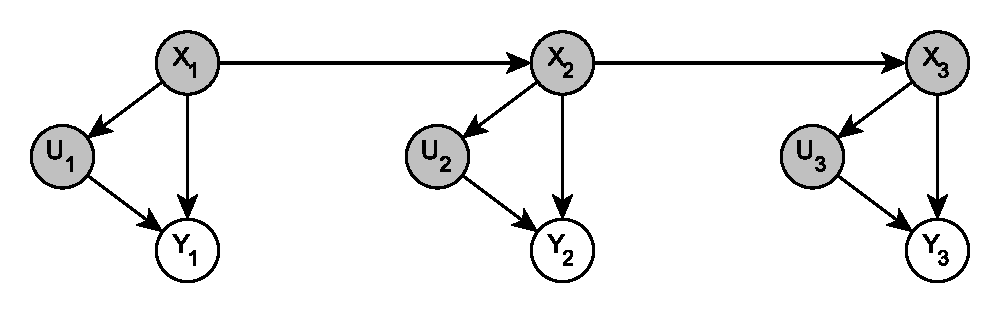
\includegraphics[scale=0.8]{general_dbn.pdf}
\caption{Example of a DBN unrolled for 3 time slices}
\label{fig_gen_dbn}
\end{figure}
To make the notation clear, the variable $X_t$ represents a Bayesian Network, for example like the arbitrary one shown in Figure \ref{fig_spec_dbn}. Similarly with $U_t$ and $Y_t$. The representation used in Figure \ref{fig_gen_dbn} is just more compact than showing the entire network as in Figure \ref{fig_spec_dbn}.
\begin{figure}[H] 
\centering
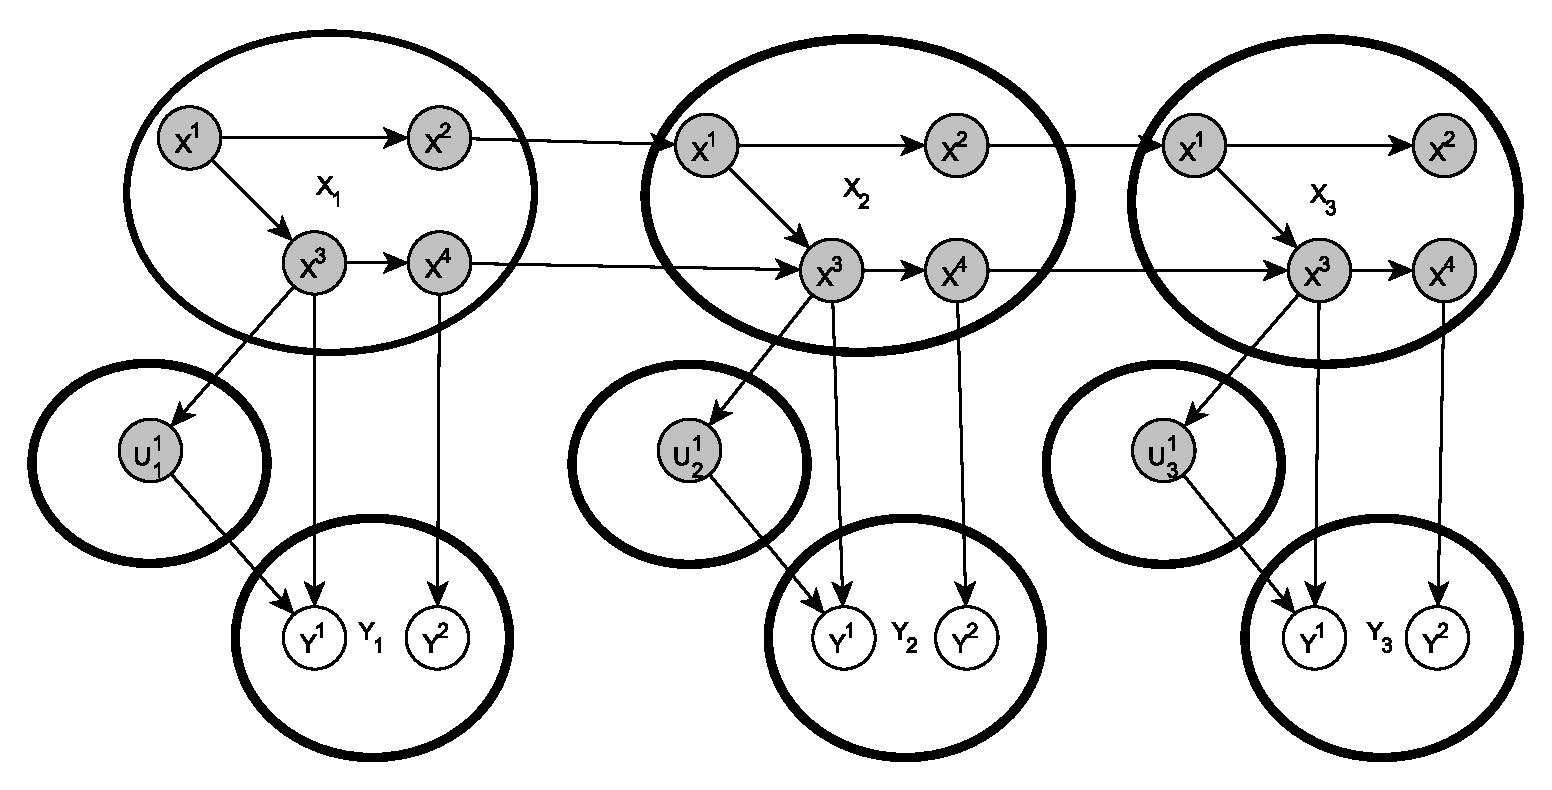
\includegraphics[scale=0.4]{spec_dbn.pdf}
\caption{Complete expanded Dynamic Bayesian Network}
\label{fig_spec_dbn}
\end{figure}

\subsection{Control}
\label{sec_lit_control}
In this section we briefly introduce three fundamental control strategies. First, the Linear Quadratic Regulator (LQR) which deals with the optimal control of linear discrete time invariant systems. Second, we deal with the stochastic generalisation of the LQR controller: the famous Linear Quadratic Gaussian (LQG) controller. Third and finally, we introduce Model Predictive Control (MPC). The aim of this section is to introduce and illustrate the relationship between these controllers.

\subsubsection{Linear Quadratic Regulator Control}
We start our analysis by assuming we have an accurate, linear, discrete, time invariant state space representation of a system shown in (\ref{eq_lqr_ss}).
\begin{equation}
\begin{aligned}
x_{t+1} &= Ax_t+ Bu_t \\
y_t &= Cx_t
\end{aligned}
\label{eq_lqr_ss}
\end{equation}
We also assume that the states are measured i.e. $C=I$ and the control sequence $N$ steps into the future is denoted $\mathbf{u}=(u_0, u_1,...,u_{N-1})$. It is our goal to derive a Linear Quadratic Regulator (controller) given the system in (\ref{eq_lqr_ss}).
\begin{defn}
\textbf{Linear Quadratic Regulator (LQR) Objective Function} The controller minimising the quadratic objective function, shown in (\ref{eq_lqr_obj}), is called the LQR controller. 
\begin{equation}
V(x_0, \mathbf{u}) = \frac{1}{2}\sum_{k=0}^{N-1} \left( x_k^TQx_k + u_k^TRu_k \right) + \frac{1}{2}x_N^TP_fx_N
\label{eq_lqr_obj}
\end{equation}
The optimisation of (\ref{eq_lqr_obj}) is implicitly subject to the state dynamics. The matrices $Q$ and $R$ are tuning parameters affecting the relative importance of the state and control inputs to the objective function respectively. We also assume that $Q, P_f$ and $R$ are real and symmetric matrices with the additional assumption that $Q, P_f$ are positive semidefinite and $R$ is positive definite.
\label{def_lqr}
\end{defn}
We assume the reader is familiar with Dynamic Programming and present Theorem \ref{thrm_lqr_q} because it will be useful later. The proof may be found in \cite{raw} and follows from algebraic manipulations.
\begin{thrm}
\textbf{Sum of Quadratics} Suppose two quadratic functions $V_1(x) = \frac{1}{2}(x-a)^TA(x-a)$ and $V_2(x) = \frac{1}{2}(x-b)^TB(x-b)$ are given. Then the sum $V_1(x) + V_2(x) = V(x)$ is also quadratic and $V(x) = \frac{1}{2}(x-v)^TH(x-v)+d$ with $H = A+B$, $v = H^{-1}(Aa+Bb)$ and $d = V_1(v) + V_2(v)$.
\label{thrm_lqr_q}
\end{thrm}
We now state the complete LQR problem for finite horizon linear systems in (\ref{eq_lqr_problem}) and analytically solve it using backward Dynamic Programming. 
\begin{equation}
\begin{aligned}
&\underset{\mathbf{u}}{\text{min }} V(x_0, \mathbf{u}) = \frac{1}{2}\sum_{k=0}^{N-1} \left( x_k^TQx_k + u_k^TRu_k \right) + \frac{1}{2}x_N^TP_fx_N \\
& \text{subject to } x_{t+1}=Ax_t+Bu_t
\end{aligned}
\label{eq_lqr_problem}
\end{equation}
Expanding the objective function to examine its structure we have (\ref{eq_lqr_expand_obj}). Note that given $x_0$ and the system dynamics all succeeding states are unknown only in the control input. The expansion of the objective function is recursive; this structure motivates the use of Dynamic Programming.
\begin{equation}
\begin{aligned}
\underset{\mathbf{u}}{\text{min }} V(x_0, \mathbf{u}) &= \underset{\mathbf{u}}{\text{min }} \frac{1}{2}\sum_{k=0}^{N-1} \left( x_k^TQx_k + u_k^tRu_k \right) + \frac{1}{2}x_N^TP_fx_N \\
&= \underset{u_0, u_1,...,u_{N-1}}{\text{min }}  \frac{1}{2}\left( x_0^TQx_0 + u_0^TRu_0 +x_1^TQx_1 + u_1^TRu_1 + ... + x_N^TP_fx_N \right) \\
&= \underset{u_0, u_1,...,u_{N-2}}{\text{min }}  \frac{1}{2}\left( x_0^TQx_0 + u_0^TRu_0 + ... + x_{N-2}^TQx_{N-2} + u_{N-2}^TRu_{N-2} \right)... \\
& \hspace{18pt} + \underset{u_{N-1}}{\text{min }} \frac{1}{2} \left(x_{N-1}^TQx_{N-1}+ u_{N-1}^TRu_{N-1} + x_N^TP_fx_N\right)
\end{aligned}
\label{eq_lqr_expand_obj}
\end{equation}
By using Theorem \ref{thrm_lqr_q} and the constraint $x_N=Ax_{N-1}+Bu_{N-1}$ we can simplify the last term in the separated minimisation problem of (\ref{eq_lqr_obj}) as shown in (\ref{eq_lqr_sum_q}). This is the first step of backward Dynamic Programming used to solve the problem.
\begin{equation}
\begin{aligned}
&\underset{u_{N-1}}{\text{min }}V_{N-1}(x_N, u_{N-1}) =\underset{u_{N-1}}{\text{min }} \frac{1}{2} \left(x_{N-1}^TQx_{N-1}+ u_{N-1}^TRu_{N-1} + x_N^TP_fx_N\right) &\\ 
&\hspace{130pt} = \underset{u_{N-1}}{\text{min }}\frac{1}{2} \left(x_{N-1}^TQx_{N-1} + (u_{N-1}-v)^TH(u_{N-1}-v)\right) + d \\
&\text{with } H = R+B^TP_fB \\
&\text{and } v = K_{N-1}x_{N-1} \\
&\text{and } d = \frac{1}{2}x_{N-1}^T\left(K_{N-1}^TRK_{N-1}+(A+BK_{N-1})^TP_f(A+BK_{N-1})  \right)x_{N-1}\\
&\text{and } K_{N-1} = -(B^TP_fB+R)^{-1}B^TP_fA
\end{aligned}
\label{eq_lqr_sum_q}
\end{equation}
Given the form of the objective function we see that the optimal input $u_{N-1}$ is $v$ and consequently that the optimal control law at time $N-1$ is a linear function, $K_{N-1}$, of $x_{N-1}$. We also see that the cost function of the last stage is quadratic. We summarise the optimal stage cost and controller action, after some simplifications, in (\ref{eq_lqr_stage1}).
\begin{equation}
\begin{aligned}
&u^0_{N-1}(x) = K_{N-1}x \\
&x^0_{N-1}(x) = (A+BK_{N-1})x \\
&V^0_{N-1}(x) = \frac{1}{2}x^T\Pi_{N-1}x \\
&K_{N-1} = -(B^TP_fB+R)^{-1}B^TP_fA \\
&\Pi_{N-1} = Q + A^TP_fA-A^TP_fB(B^TP_FB+R)^{-1}B^TP_fA 
\end{aligned}
\label{eq_lqr_stage1}
\end{equation} 
The function $V^0_{N-1}(x)$ defines the optimal cost to go from state $x$ for the last stage under the optimal control law $u^0_{N-1}(x)$. Now we proceed with the backward Dynamic Programming and solve (\ref{eq_lqr_stage2_obj}).
\begin{equation}
\underset{u_{N-2}}{\text{min }}  \frac{1}{2}\left(x_{N-2}^TQx_{N-2} + u_{N-2}^TRu_{N-2} \right) + V^0_{N-1}(x_{N-1})
\label{eq_lqr_stage2_obj}
\end{equation}
But now we note the similarity between (\ref{eq_lqr_sum_q}) and (\ref{eq_lqr_stage2_obj}). Using $x_{N-1}=Ax_{N-2}+Bu_{N-2}$ and the same procedure as before we have (\ref{eq_lqr_stage2}). 
\begin{equation}
\begin{aligned}
&u^0_{N-2}(x) = K_{N-2}x \\
&x^0_{N-2}(x) = (A+BK_{N-2})x \\
&V^0_{N-2}(x) = \frac{1}{2}x^T\Pi_{N-2}x \\
&K_{N-2} = -(B^T\Pi_{N-1}B+R)^{-1}B^T\Pi_{N-1}A \\
&\Pi_{N-2} = Q + A^T\Pi_{N-1}A-A^T\Pi_{N-1}B(B^T\Pi_{N-1}B+R)^{-1}B^T\Pi_{N-1}A 
\end{aligned}
\label{eq_lqr_stage2}
\end{equation} 
The recursion to go from $\Pi_{N-1}$ to $\Pi_{N-2}$ is known as backward Ricatti iteration and is defined in (\ref{eq_ricatti}).
\begin{equation}
\Pi_{k-1} = Q + A^T\Pi_{k}A-A^T\Pi_{k}B(B^T\Pi_{k}B+R)^{-1}B^T\Pi_{k}A  
\label{eq_ricatti}
\end{equation}
With terminal condition $\Pi_N = P_f$. We see that to find the optimal control policy we need to continue with the backward Dynamic Programming recursion relationships until $k = 1$. We summarise one of the most fundamental results in Optimal Control theory in Theorem \ref{thrm_lqr_sol}.
\begin{thrm}
\textbf{Solution of the Finite Horizon LQR control problem} Given a finite horizon $N$ and a discrete linear system as shown in (\ref{eq_lqr_ss}) the optimal control policy which minimises the LQR objective function of defintion \ref{def_lqr} is given by iterating (\ref{eq_lqr_opt_control}) backwards for $k=N-1, N-2, ..., 1$ using backward Ricatti iteration as shown in (\ref{eq_ricatti}). 
\begin{equation}
\begin{aligned}
&u^0_{k}(x) = K_{k}x \\
&K_k = -(B^T\Pi_{k+1}B+R)^{-1}B^T\Pi_{k+1}A
\end{aligned}
\label{eq_lqr_opt_control}
\end{equation}
The optimal cost to go from time $k$ to time $N$ is $V^0_{k}(x)=\frac{1}{2}x^T\Pi_{k}x$.
\label{thrm_lqr_sol}
\end{thrm}
After the optimal input $\mathbf{u}$ is found only $u_0$ is applied. For a treatment of the continuous case see \cite{robust}.

Unfortunately optimal control in the setting described above does not guarantee stable control \cite{raw}. It can be shown that the finite horizon controller is not guaranteed to be stable i.e. there exist non-trivial systems for which the controller is unstable. This problem is fixed by considering the infinite horizon LQR problem. 
\begin{defn}
\textbf{Infinite Horizon LQR problem} Find the optimal control sequence $\mathbf{u}$ which solves (\ref{eq_inf_lqr_problem}).
\begin{equation}
\begin{aligned}
&\underset{\mathbf{u}}{\text{min }} V(x, \mathbf{u}) = \frac{1}{2}\sum_{k=0}^{\infty} \left( x_k^TQx_k + u_k^TRu_k \right) \\
&\text{subject to } x_{t+1} = Ax_t+Bu_t \\
&\text{and } x_0 = x
\end{aligned}
\label{eq_inf_lqr_problem}
\end{equation}
The same restrictions on the tuning parameters apply as before.
\label{def_inf_lqr}
\end{defn}
By assuming that the system under consideration is controllable it is possible to show that the infinite horizon LQR solution shown in Theorem \ref{thrm_lqr_inf} is convergent and stabilising.
\begin{defn}
\textbf{Controllability} A system is controllable is, for any pair of states $x,z$ in the state space, $z$ can be reached in finite time from $x$. That is, $x$ can be controlled to $z$. It is possible to characterise a controllable system further. A system with $n$ variables (which require control) is controllable if and only if $\text{rank}\begin{pmatrix}
\lambda I- A & B
\end{pmatrix} = n$ for all $\lambda \in \text{eig}(A)$. 
\end{defn}
\begin{thrm}
\textbf{Solution of the Infinite Horizon LQR control problem} Given the Infinite Horizon LQR problem of definition \ref{def_inf_lqr} it can be shown that the optimal control is given by (\ref{eq_lqr_inf_opt_control}).
\begin{equation}
\begin{aligned}
&u^0_{k}(x) = Kx \\
&K = -(B^T\Pi B+R)^{-1}B^T\Pi A \\
&\Pi = Q + A^T\Pi A-A^T\Pi B(B^T\Pi B+R)^{-1}B^T\Pi A  
\end{aligned}
\label{eq_lqr_inf_opt_control}
\end{equation}
The optimal cost is given by $V^0(x) = \frac{1}{2}x^TKx$. The matrix $\Pi$ can be found by iterating the Ricatti equation. This solution is stabilising if the system is controllable.
\label{thrm_lqr_inf}
\end{thrm}
The LQR control problem, as discussed in this section, applies to deterministic systems where the goal is to drive the controlled variables to the origin. It is straightforward to extend this approach to systems where it is desired to drive the states to a reference (set) point $r_{sp}$.

To achieve this we simply redefine the objective function in terms of deviation variables as shown in (\ref{eq_dev_vars}). The constants $x_{sp}$ and $u_{sp}$ are the state set point and corresponding controller set point one would like to drive the system to.
\begin{equation}
\begin{aligned}
&\tilde{x}_t = x_t-x_{sp} \\
&\tilde{u}_t = u_t-u_{sp}
\end{aligned}
\label{eq_dev_vars}
\end{equation} 
The deviation variables are then used in the objective function as opposed to $x_t$ and $u_t$ as shown in (\ref{eq_lqr_problem_dev}). Note that the system dynamics remain the same \cite{raw}. 
\begin{equation}
\begin{aligned}
&\underset{\tilde{\mathbf{u}}}{\text{min }} V(x_0, \tilde{\mathbf{u}}) = \frac{1}{2}\sum_{k=0}^{N-1} \left( \tilde{x}_k^TQ\tilde{x}_k + \tilde{u}_k^TR\tilde{u}_k \right) + \frac{1}{2}\tilde{x}_N^TP_f\tilde{x}_N \\
& \text{subject to } \tilde{x}_{t+1}=A\tilde{x}_t+B\tilde{u}_t
\end{aligned}
\label{eq_lqr_problem_dev}
\end{equation}
As before only $\tilde{u}_0$ is used. We apply $u_0 = \tilde{u}_0 + u_{sp}$ to the system. All that is required is that we specify $x_{sp}$ and $u_{sp}$. This is done by solving (\ref{eq_setpoints}). Note that $H$ relates the observed variables to the controlled variables.
\begin{equation}
\begin{pmatrix}
I-A &- B \\ HC & 0
\end{pmatrix} \begin{pmatrix}
x_{sp}\\u_{sp}
\end{pmatrix} = \begin{pmatrix}
0 \\ r_{sp}
\end{pmatrix}
\label{eq_setpoints}
\end{equation}
It is possible to cast (\ref{eq_setpoints}) into an optimisation problem if there are more controlled variables than inputs. We refer the reader to \cite{raw} for a full treatise on the subject.
 
\subsubsection{Linear Quadratic Gaussian Control}
The LQR problem dealt with deterministic systems where the states were known exactly. However, this is problematic from a practical perspective because:
\begin{enumerate}
\item
The system model is almost never known exactly.
\item
The state measurements are almost always noisy.
\end{enumerate}
The Linear Quadratic Gaussian (LQG) controller deals with a performance measure for stochastic systems of the form (\ref{eq_lqg_ss}).
\begin{equation}
\begin{aligned}
x_{t+1} &= Ax_t+ Bu_t + w_t \\
y_t &= Cx_t +v_t \\
\end{aligned}
\label{eq_lqg_ss}
\end{equation}
With  $w_t \sim \mathcal{N}(0, W)$ and $v_t \sim \mathcal{N}(0, V)$ which are independent white noise terms. 
Because the states and measurements are stochastic variables we cannot use the LQR objective function as before. Instead we use the LQG objective function which is a generalisation of the former as shown in definition \ref{def_lqg_obj}.
\begin{defn}
\textbf{Linear Quadratic Gaussian (LQG) Objective Function} The controller minimising the quadratic objective function, shown in (\ref{eq_lqg_obj}), is called the LQG controller. 
\begin{equation}
V(x_0, \mathbf{u}) = \mathbb{E}\left[ \frac{1}{2}\sum_{k=0}^{N-1} \left( x_k^TQx_k + u_k^TRu_k \right) + \frac{1}{2}x_N^TP_fx_N \right]
\label{eq_lqg_obj}
\end{equation}
The restrictions on the tuning parameters are the same as before.
\label{def_lqg_obj}
\end{defn}
The full LQG control problem is stated in (\ref{eq_lqg_problem}). Note that we only observe noisy $y_t$ and that $C \neq I$ in general.
\begin{equation}
\begin{aligned}
&\underset{\mathbf{u}}{\text{min }} V(x_0, \mathbf{u}) = \mathbb{E}\left[ \frac{1}{2}\sum_{k=0}^{N-1} \left( x_k^TQx_k + u_k^TRu_k \right) + \frac{1}{2}x_N^TP_fx_N \right] \\
& \text{subject to } x_{t+1}=Ax_t+Bu_t + w_t \\
& \text{and } y_{t}= Cx_t + v_t \\
\end{aligned}
\label{eq_lqg_problem}
\end{equation}

It is indeed possible to solve this controller analytically using stochastic Dynamic Programming but the derivation is tedious. We rather employ the Separation Principle \cite{lqg}. We do however re-derive the optimal controller in a later section.
\begin{defn}
\textbf{Separation Principle} The solution of the LQG problem is obtained by combining the solution of the deterministic LQR problem and the optimal state estimation problem. The optimal current state estimate is used as the current deterministic state within the framework of the LQR controller. 
\end{defn}
The optimal state estimate of linear systems under Gaussian noise is known as the Kalman Filter. In later sections we devote much time to its derivation but for now we merely introduce it loosely.
\begin{defn}
\textbf{Kalman Filter} Given a linear system like (\ref{eq_lqg_ss}) under the influence of white Gaussian noise, the Kalman Filter is the optimal state estimator.
\end{defn}
A schematic diagram of the solution of LQG control problem is shown  in Figure \ref{fig_lqg}.
\begin{figure}[H] 
\centering
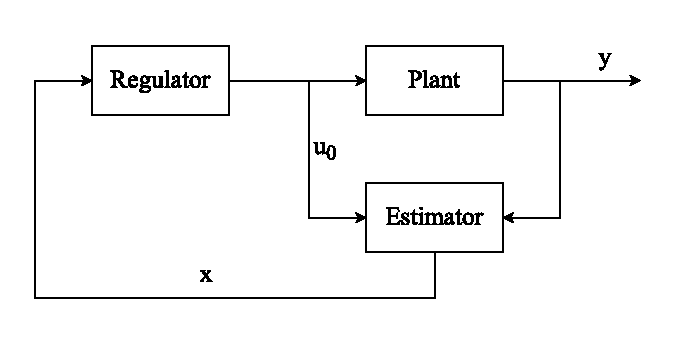
\includegraphics[scale=1.0]{LQG.pdf}
\caption{LQG control schematic}
\label{fig_lqg}
\end{figure}
The LQR and LQG controllers are two of the most fundamental results in Optimal Control theory \cite{robust}. In the next section we discuss Model Predictive Control (MPC) which is a generalisation of the controllers we have discussed so far.

\subsubsection{Model Predictive Control}
Model Predictive Control
